% vim: set textwidth=78 autoindent:

\section{Koordinaten abgreifen Plugin}\index{Plugins!Koordinaten abgreifen}

% when the revision of a chapter has been finalized, 
% comment out the following line:
% \updatedisclaimer

Das Plugin \toolbtntwo{coordinate_capture}{Koordinaten abgreifen} ist einfach
zu bedienen und erlaubt es, mit der linken Maustaste Koordinaten f�r zwei
ausgew�hlte Koordinatenbezugssysteme (KBS) im Kartenfenster abzufragen. 

\begin{figure}[ht]
   \begin{center}
   \caption{Koordinaten abgreifen Dialog \nixcaption}
   \label{fig:coordinate_capture_dialog}\smallskip
   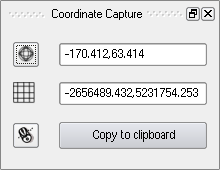
\includegraphics[clip=true, width=8cm]{coordinate_capture_dialog}
\end{center}  
\end{figure}

\begin{enumerate}
  \item Starten Sie QGIS, w�hlen Sie
\dropmenuopttwo{mActionOptions}{Projekteinstellungen} im Men�
\mainmenuopt{Einstellungen} und klicken Sie auf den Reiter
\tab{Benutzerkoordinatenreferenzsystem}. Alternativ klicken Sie das
\toolbtntwo{mIconProjectionDisabled}{KBS Status} Icon in der unteren rechten
Ecke der Statusleiste.
  \item Aktivieren Sie das Kontrollk�stchen
\checkbox{On-the-Fly-KBS-Transformation aktivieren} und w�hlen Sie ein KBS
Ihrer Wahl (siehe dazu auch Kapitel~\ref{label_projections}).
  \item Laden Sie nun das Koordinaten abgreifen Plugin (vgl.
Kapitel~\ref{sec:load_core_plugin}) und klicken das
\toolbtntwo{coordinate_capture}{Koordinaten abgreifen} Icon. Der Dialog
wie in Abbildung~\ref{fig:coordinate_capture_dialog} erscheint.
  \item Klicken Sie nun auf das Icon \toolbtntwo{geographic}{Klicken Sie, um
das KBS zur Koordinatenanzeige auszuw�hlen} und w�hlen Sie anderes
Koordinatenbezugsystem (KBS) als eben.
  \item Sie k�nnen nun auf einen Punkt im Kartenfenster klicken und das
Plugin zeigt ihnen die Koordinaten f�r diesen Punkt in beiden zuvor gew�hlten
KBS an (siehe Abbildung~\ref{fig:coordinate_capture_dialog}).
  \item Um die Mausverfolgungs-Funktion zu starten, klicken Sie auf das Icon
\toolbtntwo{tracking}{Mausverfolgung}.
  \item Sie k�nnen die ausgew�hlten Koordinaten auch in die Zwischenablage
kopieren.
\end{enumerate}

\newpage


